\section{On-accelerator training framework} \label{sec:framework}
In contrast to the typical offline training framework on GPPs, we propose an 
on-accelerator training framework to allow the CNN accelerator's runtime variation 
caused by approximate arithmetic logic, overclocking or soft errors 
to be learned with the application data. With the on-accelerator training,
the obtained model can be deployed despite the accelerator's 
undeterministic behavior. Details of the framework will be presented in 
the rest of this section.

\subsection{Overall training framework}
The on-accelerator training is essentially to have the neural 
network models to tolerate the accelerators' dynamic variation. 
While the variation is similar to the quantization 
errors in certain extent, the ideal network model can be 
close to the pretrained neural network model in terms of 
network structure. In this case, we borrow the idea of knowledge 
distilling\cite{distillation_38, distillation_39}, 
which can be used to have a high-precision neural network to teach a 
low-precision neural network with similar network structure efficiently, 
for the on-accelerator training. Basically, the offline pretrained 
model can be taken as a teacher model and used to guide the training of the 
student model with lower precision. After the training, the student model 
can perform much better despite the accelerators' computing variation.

\begin{figure*}
        \center{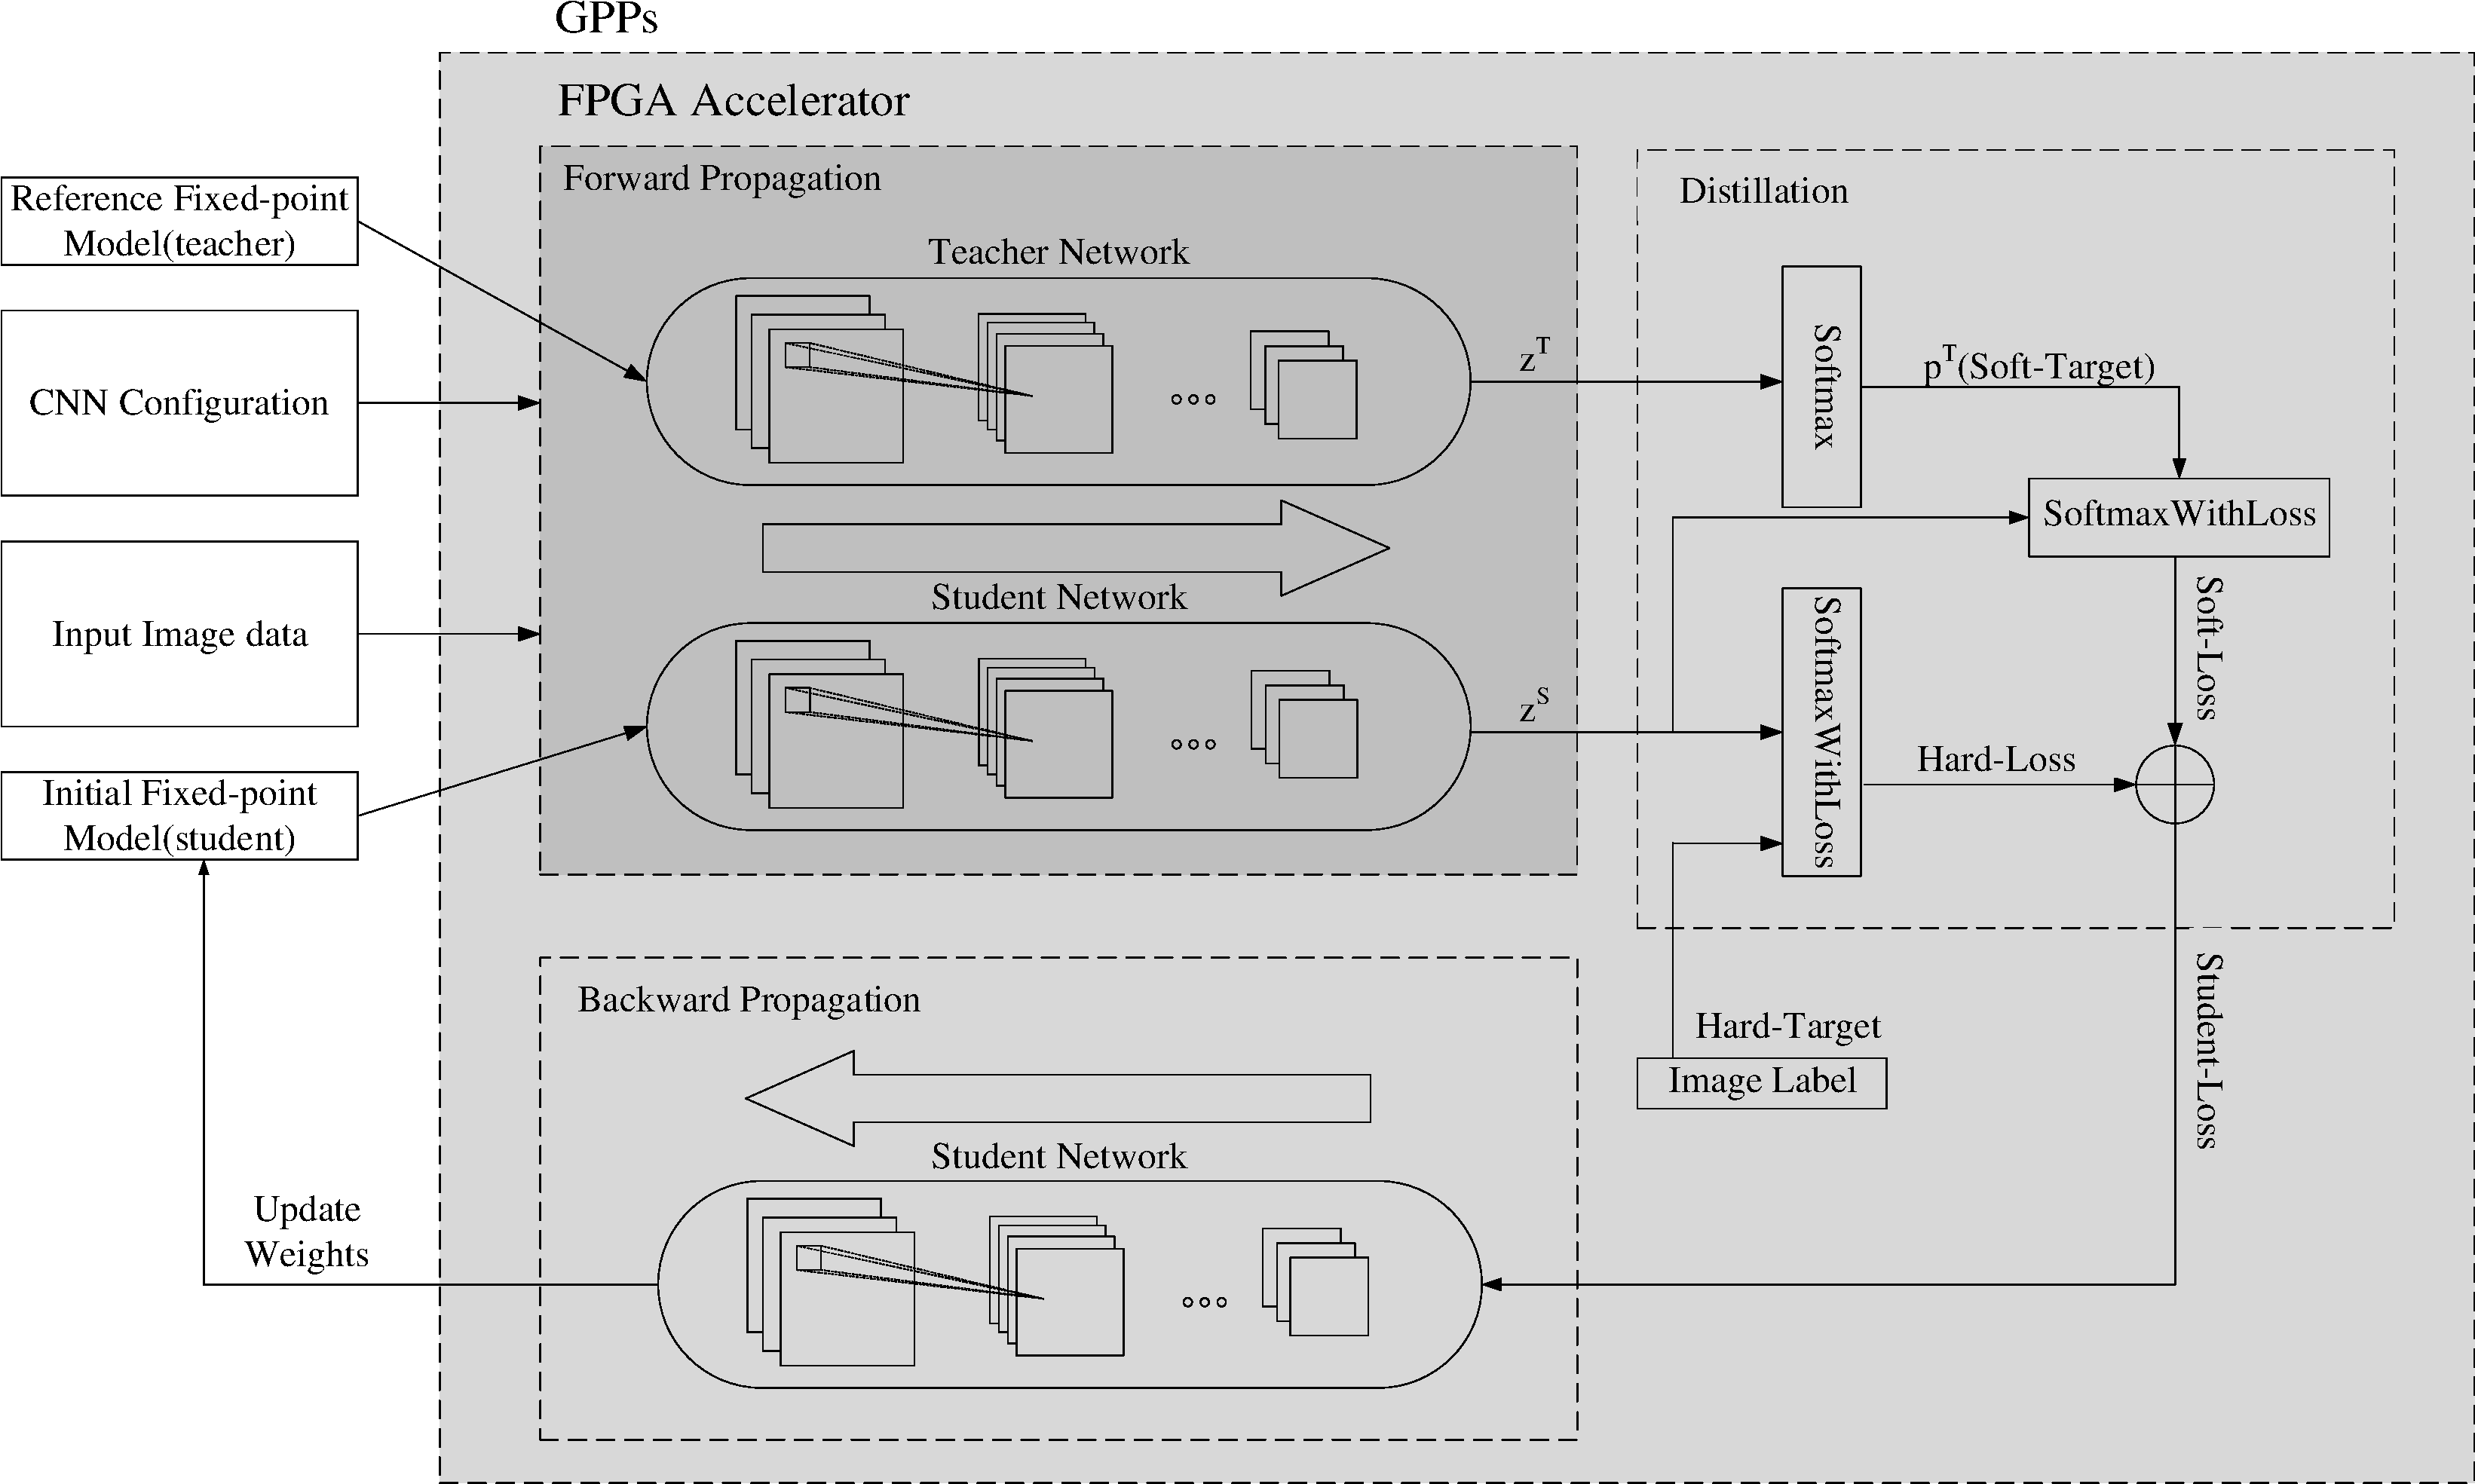
\includegraphics[width=0.85\linewidth]{retrain}}
        \caption{On-accelerator training framework with knowledge distilling}
        \label{fig:retrain}
%        \vspace{-0.5em}
\end{figure*}


With the knowledge distilling strategy, we develop an on-accelerator training 
framework as illustrated in Figure 3. The framework roughly consists of three parts
including forward propagation, knowledge distilling and backward propagation. 
Both the teacher network and the student network will go through the 
forward propagation. The computing results i.e. $z^T$ and $z^S$ in 
combination with the label of the input image data will be fed to the 
knowledge distilling part. In the knowledge distilling part,  
the logit of softmax i.e. $z^T$ and $z^S$ are further used to calculate the 
softmax i.e. $p^T$ and $p^S$ with Equation \ref{eq:pt-calu}. 
Note that the logit of the teacher network is divided by a 
temperature factor t. It can be used to adjust the softmax 
probability distribution. Using a higher value for t 
produces a softer probability distribution and stresses 
the training process. 

On top of the softmax, we can further calculate the student 
network loss with Equation \ref{eq:student-loss}. It includes 
two different parts i.e.$L(y, p^S)$ and $L(p^T, p^S)$ which can be 
obtained with Equation \ref{eq:loss}. The student loss is used in the 
back propagation part as conventional neural network training. 
After the back propagation, weights will be updated and used for the 
next training iteration. The training will stop when the prediction 
accuracy gets converged.

\begin{equation}
	\label{eq:pt-calu}
p_j=\frac{e^{{z_j}/t}}{\sum_{i=1}^{K}e^{{z_i}/t}}
\end{equation}

\begin{equation}
	\label{eq:student-loss}
L=\alpha*L(y,p^S)+\beta*L(p^T,p^S)
\end{equation}

\begin{equation}
	\label{eq:loss}
L(y,p)=-\sum_{i=1}^{K}y_i*log(p_i)
\end{equation}


To make the training aware the accelerators' dynamic variation, 
we have the forward propagation of the student network 
performed on the accelerator directly while the rest of the 
framework remains on GPPs. While the forward propagation on 
the accelerator is fixed point, the backward propagation on 
GPPs adopts the floating point to ensure 
the small change in the gradient can be accumulated \cite{Matthieu2014_8}. 


\subsection{CNN accelerator abstraction}
As illustrated in the above section, the forward propagation of the 
student network will be executed on the CNN accelerator FPGAs while 
the rest part runs on GPPs. Essentially, the framework targets at a 
heterogeneous computing architecture and there are frequent 
communication between the accelerator and the GPPs. 
With the growing popularity of deep learning, massive different 
CNN accelerators have been developed. 
In order to fit various CNN accelerators within the same training framework,
we abstract the CNN accelerators.

To that end, we define a set of high-level interface functions
centering the data communication between the forward propagation part 
and the rest of the training framework. The interface functions are listed 
in Table 1 and 7 functions are included. Function 1 is used to launch the CNN accelerator from host. 
Function 2 and 3 are used to transfer data between the host memory and the device memory during 
the training. As the forward propagation on the CNN accelerators is usually fixed point 
and the back propagation on GPPs is floating point, data type converting between fixed point 
and floating point is required. Function 4 and 5 can be used for this purpose. 
Function 1 to 5 are required for all the accelerators. 
Function 6 and 7 are only used for accelerators that compute on reorganized data\cite{pipecnn_2,deepburing_12}. 
With the interface functions, general CNN accelerators can be conveniently 
referenced and used in the proposed on-accelerator training framework. 


In this work, we have the CNN accelerator implemented on Xilinx FPGAs as a case study. 
The accelerator can either be realized with high-level synthesis tools (HLS) or 
hardware description languages (HDL). With Xilinx SDAccel, we can wrap both 
styles of accelerators with OpenCL API. Given the OpenCL API,  
the proposed interface functions can be implemented and referenced conveniently. 
We choose Caffe, a C++ based deep learning framework, to construct the on-accelerator training framework.  

\begin{table*}
        \centering
        \vspace{-0.3em}
        \caption{High-level interface to integrate general CNN accelerators with Caffe}
        \label{tab:graph}
        \vspace{-0.3em}
        \begin{tabular}{c|l|l}
                \toprule
                ID & Function Name & Description  \\
                \midrule
                1 & launchAccelerator() & It configures the CNN accelerator and launches it from host CPU. \\
		\midrule
                2 & dataToFPGA(weight, input, wgtDevAddr, inDevAddr) & It transfers both the input data and weight to the FPGA device memory. \\
		\midrule
		3 & dataFromFPGA(outputDevAddr, output) & \shortstack[l]{It transfers all the intermediate output of the CNN layers from FPGA \\device memory to host memory.} \\
		\midrule
		4 & convertIntToFloat(int iData, float fData) & It converts the fixed-point output to float for back propagation processing. \\
		\midrule
		5 & convertFloatToInt(float fData,  int iData) & \shortstack[l]{It converts the floating-point input and weight data to fixed point or \\integer for forward processing on the accelerator.} \\
		\midrule
		6 & dataLayoutReorder(data, reorderedData) & \shortstack[l]{It reorders the data layout for more efficient accelerator execution before \\sending to FPGA device memory.} \\
		\midrule
		7 & dataLayoutRecover(reorderedData, data) & It reorders the output data back to the default format for Caffe back propagation. \\
                \bottomrule
        \end{tabular}
        \vspace{-1em}
\end{table*}
In this work, we have the CNN accelerator implemented on FPGAs.
Figure 4 depicts the implementation of the training framework on a hybrid 
CPU-FPGA architecture. In this work, we use Xilinx KCU1500 as the FPGA board 
and put it on a standard desktop computer. CPU is the controller and it reconfigures 
the accelerator for a specific CNN structure. In each training iteration, CPU launches 
the CNN accelerator to perform the forward propagation from bottom layer to top layer. 
CPU does the backward propagation from top layer to bottom layer. Weights and the image 
data are initially stored in host memory. It will be transferred to FPGA offchip memory 
for forward propagation through PCI-E. Similarly, the output data will be transferred 
from FPGA off-chip memory back to host memory after forward propagation. Because of the 
OpenCL based API wrapper in SDAccel, the CNN accelerator’s interface can be easily 
exposed to Caffe for referring to the forward propagation result. 


\subsection{CNN accelerator modification}
  On top of the interface, the CNN accelerator also needs minor adjustment for the training. 
The training process requires the feature maps of each CNN layer for backward propagation, 
while the accelerators are typically optimized for inference and some of the layers’ output 
are fully buffered in on-chip memory for less memory access overhead. In this case, 
the accelerator should make intermediate output write back optional as shown in Figure 5. 
When the accelerator is used in training, the output will be transferred to memory. 
When it is used for inference, it can also turn off the write back data path for better performance. 
It is trivial to modify the CNN accelerators and the hardware overhead is negligible.

\begin{figure}
        \center{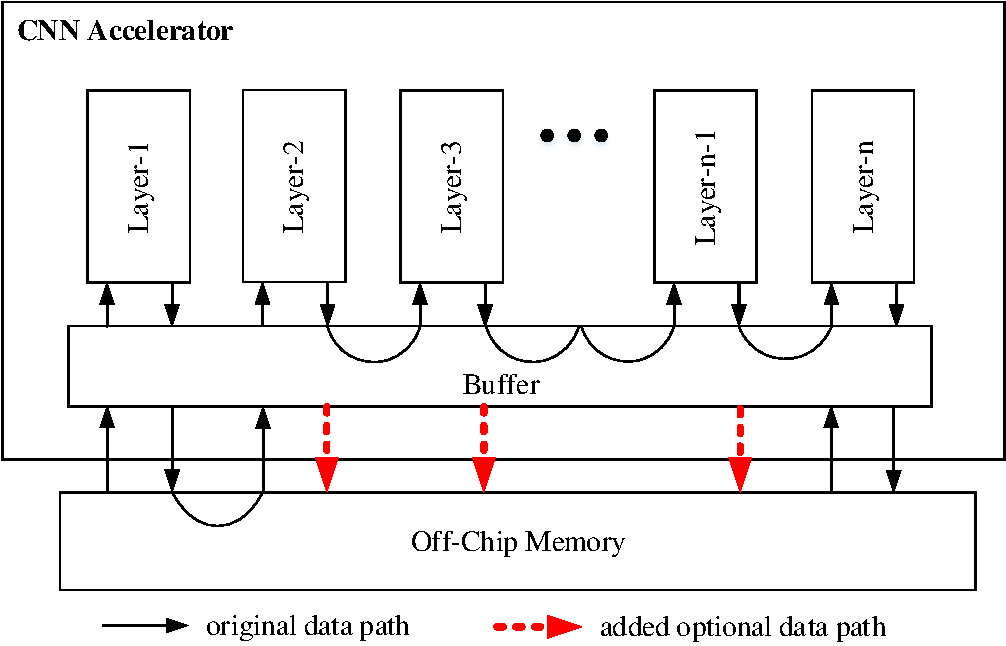
\includegraphics[width=0.85\linewidth]{change_of_accelerator}}
        \caption{Modification of the CNN accelerator data path. It essentially
ensures each CNN layer to have an optional data path to off-chip memory so that it
can be used for training as necessary.}
        \label{fig:change_of_accelerator}
        \vspace{-1em}
\end{figure}


